\section{Problem specification}

The basic input of the deconflicting problem is a set of ideal flight trajectories (space-time paths).
These ideal trajectories are specified by the individual flight operators.
Each ideal trajectory represents some independent optimization from the operator's perspective, especially minimizing fuel costs given expected wind conditions between the desired origin and destination at the desired times;
for this reason, they are called the ``wind-optimal'' trajectories.
Because of the number of such trajectories and the correlation between them, these trajectories are likely to conflict; that is, two or more aircraft are likely to get dangerously close to each other if their ideal trajectories are followed without modification.
The goal thus is to modify the trajectories to avoid such conflicts.

In theory, the configuration space consists of all physically realistic trajectories; in practice, computational bounds constrain us to consider perturbations of the ideal trajectories.
The simplest such perturbation is a departure delay, which is the main focus of the present work.
Previous work~\cite{rodionova16} additionally considered a global perturbation by which a trajectory is sinusoidally shifted parallel to the Earth's surface.
We focus instead on local perturbations to the trajectories, in which a modification to the trajectory is parameterized by some choice of active maneuvers near a potential conflict; such a modification does not affect the preceding part of the trajectory and only affects the subsequent part by the additional delay it introduces.

A full accounting of the cost of such modifications would take into account the cost of departure delays, the change in fuel cost due to perturbing the trajectories, the relative importance of each flight, and many other factors.
As in previous work, we consider only the total, unweighted arrival delay, aggregated equally over all of the flights.

Formally, each ideal trajectory $\mathbf x_i = {\left(x_{i, t}\right)}_{t=t_{i,0}}^{t_{i,1}}$ is specified as a time-discretized path from the departure point $x_{i, t_{i, 0}}$ at time $t_{i, 0}$ to the arrival point $x_{i, t_{i, 1}}$ at time $t_{i, 1}$.
For each flight $i$, the geographical coordinates $x_{i,t}$ (as latitude, longitude, and altitude) are specified at every unit of time (i.e.\ one minute) between $t_{i,0}$ and $t_{i,1}$;
we call this interval $T_i = \left(t_{i,0}, t_{i, 0} + 1, \ldots, t_{i,1}\right)$.

For notational simplicity, suppose momentarily that each trajectory $\mathbf x_i$ is modified only by introducing delays between time steps.
Let $\delta_{i, t}$ be the accumulated delay of flight $i$ at the time that it reaches the point $x_{i, t}$, and let $\delta^*_{i, t}$ be the maximum such delay.

A pair of flights $(i, j)$ are in conflict with each other if any pair of points from their respective trajectories is in conflict.
(The trajectories are reasonably assumed to be sufficiently time-resolved so that if the continuously interpolated trajectories conflict than there is a pair of discrete trajectory points that conflict.)
A pair of trajectory points $(x_{i,s}, x_{j,t})$ conflict if their spatial and temporal separations are both within the respective mandatory separation standards $\Delta_x$ and $\Delta_t$ (i.e.\ $3$ nautical miles and $3$ minutes):
\begin{equation}
\left\|x_{i, s} - x_{j,t}\right\| < \Delta_x \text{ and } 
\left|\left(s + \delta_{i, s}\right) - \left(t + \delta_{j,t}\right)\right|
\end{equation}.
The latter condition can be met for some 
$\left(\delta_{i,s}, \delta_{j,t} \right) \in [0, \delta^*_{i,s}] \times [0, \delta^*_{j,t}]$ if and only if 
\begin{equation}
\max \left\{\delta^*_{i, s}, \delta^*_{j, t}\right\} + \Delta_t > |s - t|,
\end{equation}
in which case we call the pair of trajectory points \emph{potentially} conflicting.
The set $C$ of such pairs of potentially conflicting trajectory points contains strongly correlated clusters.
To simplify the constraints, we enumerate all such clusters and refer to them simply as \emph{the} conflicts.
That is, we partition the potentially conflicting pairs of trajectory points into disjoint sets,
\begin{equation}
C =  \bigcup_{k} C_k,
\end{equation}
such that if $\left\{(i, s), (j, t)\right\}, \left\{(i', s'), (j', t')\right\} \in C_k$ for some $k$ then
$i = i' < j = j'$ and for all 
$s'' \in [\min \{s, s'\}, \max\{s, s'\}]$
there exists some 
${t'' \in [\min \{t, t'\}, \max\{t, t'\}]}$
such that
${\left\{(i, s''), (j, t'')\right\} \in C_k}$.
Thus every conflict $k$ is associated with a pair of flights $I_k = \{i, j\}$.
Let $K_i = \left\{k \middle| i \in I_k \right\}$ be the set of conflicts to which flight $i$ is associated.

Having identified disjoint sets of conflicts, we relax the supposition that the trajectory modifications only introduce delays between time steps.
Instead, we consider modifications to the trajectories that introduce delays local to particular conflicts.
Specifically, the configuration space consists of the departure delays $\mathbf d = {\left(d_i\right)}_{i=1}^n$ and the set of local maneuvers $\mathbf a_{\mathbf k} = {\left(\mathbf a_k\right)}_k$, where $\mathbf a_k$ represents some parameterization of the local maneuvers used to avoid conflict $k$.
Let $d_{i, k} (\mathbf d, \mathbf a_{\mathbf k})$ be the delay introduced to flight $i$ at conflict $k$, as a function of the departure delays and local maneuvers.
With this notation, we can write the total delay as
\begin{equation}
D = 
\sum_{i = 1}^{n}
\left(d_i + \sum_{k \in K_i} d_{i, k}\right).
\end{equation}
This is the quantity we wish to minimize subject to avoiding all potential conflicts.
\begin{figure}[t]
    \begin{center}
        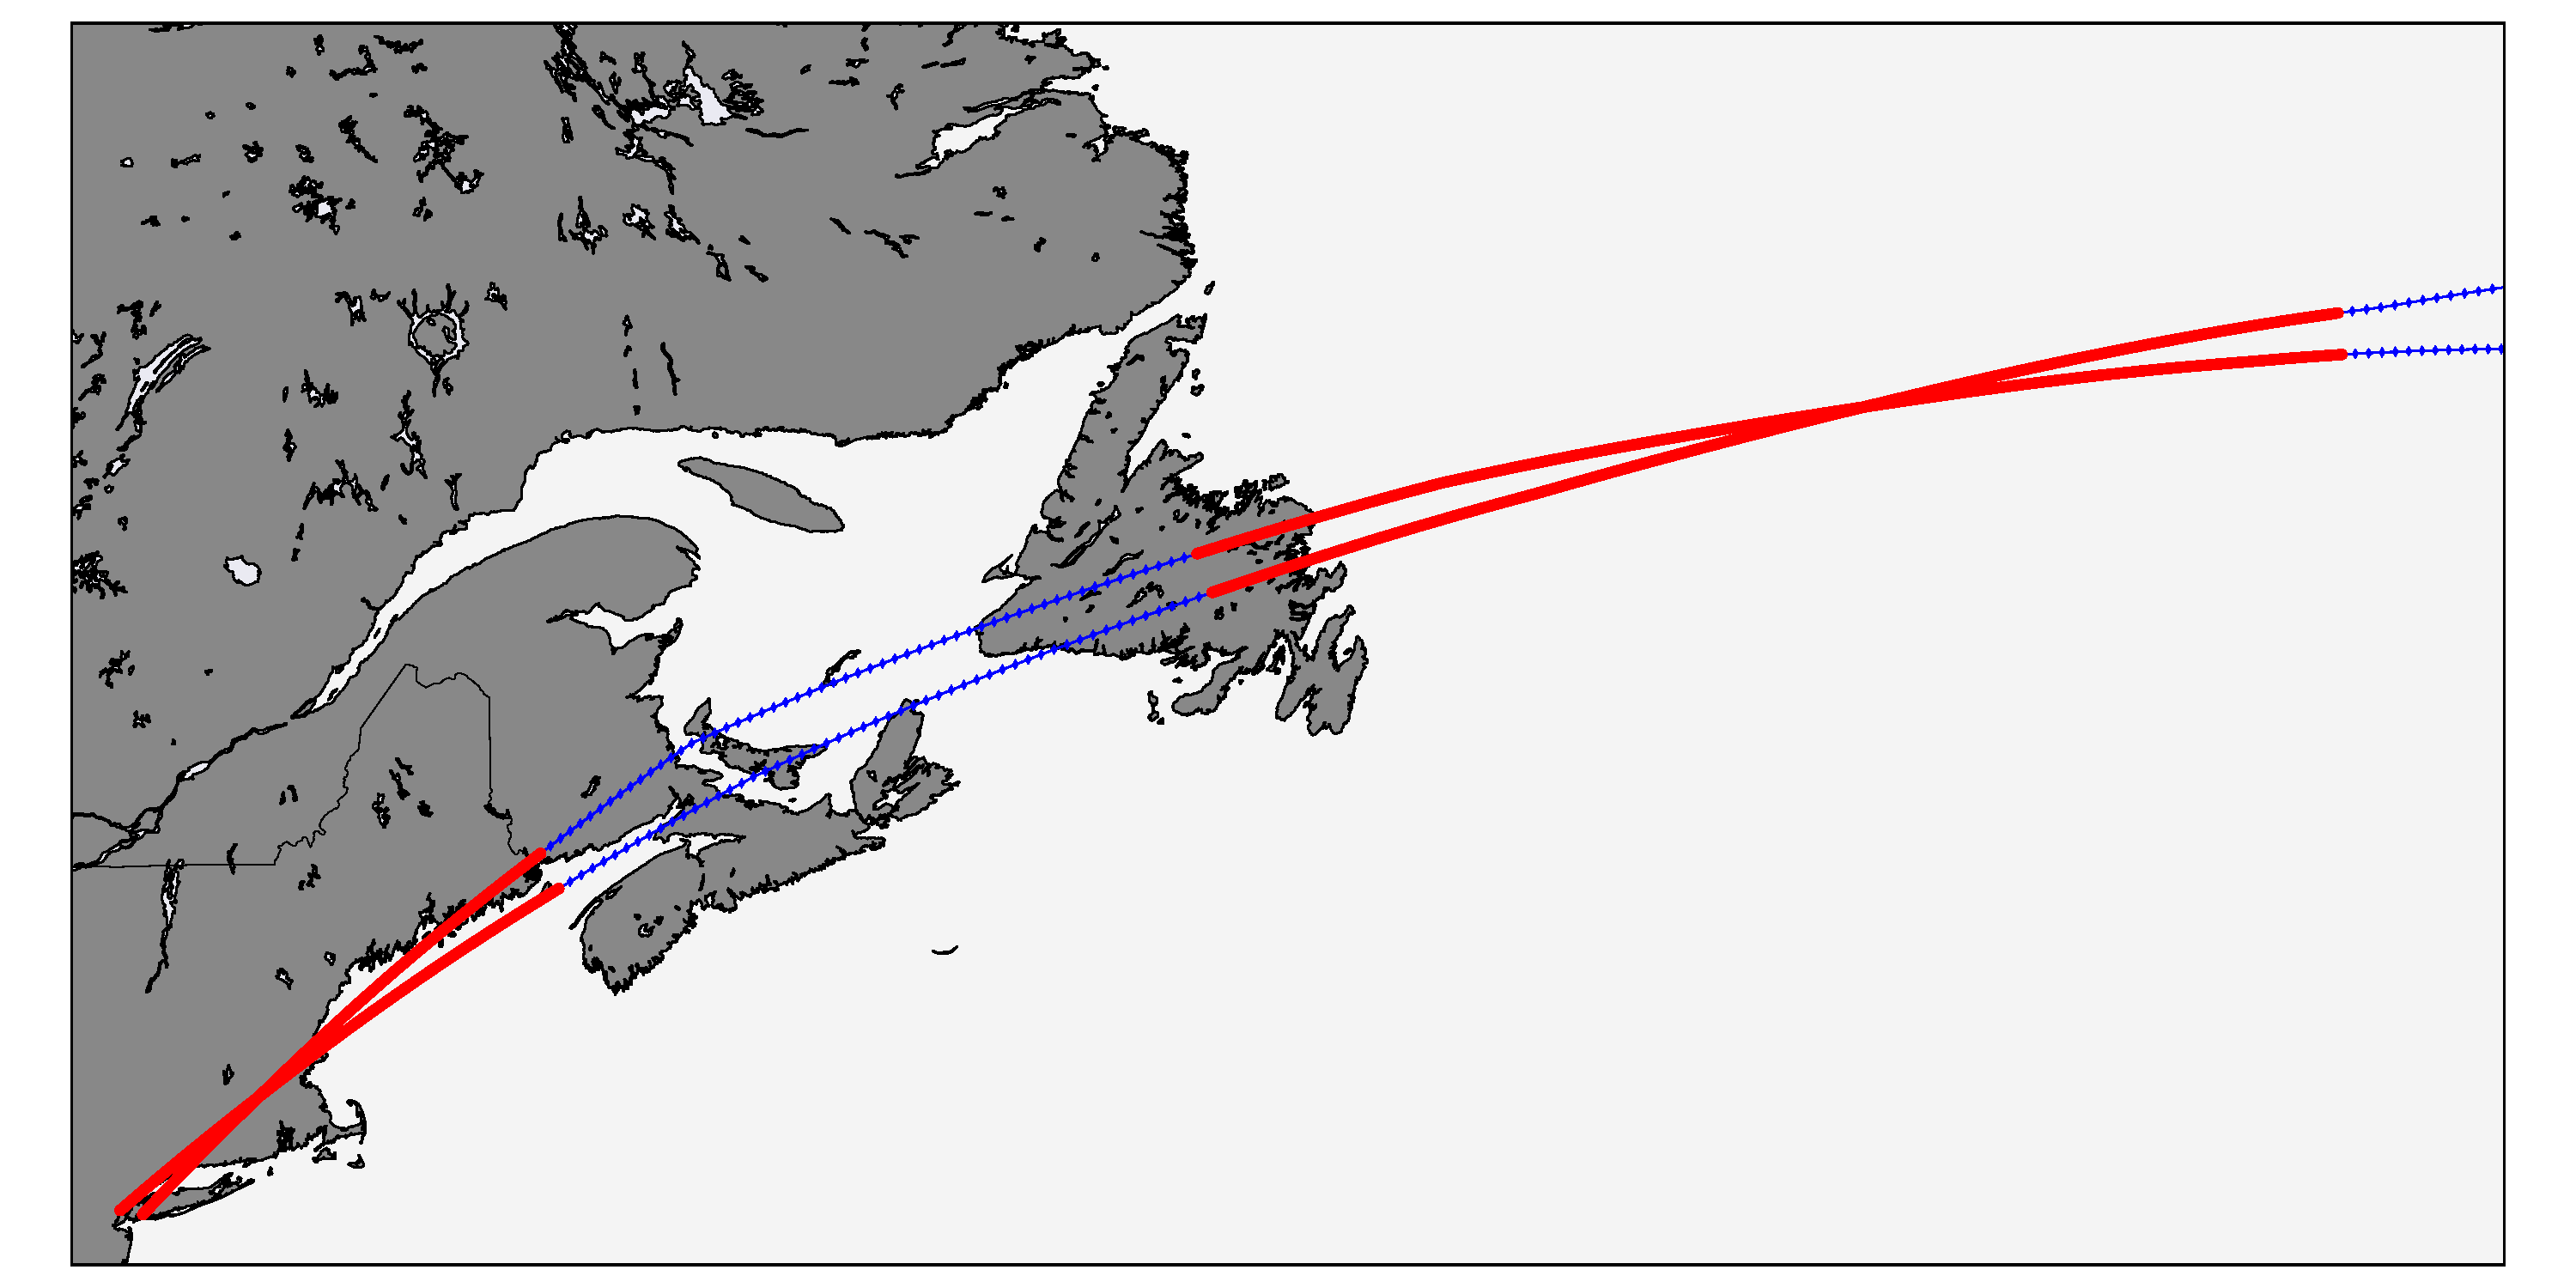
\includegraphics[width=0.45\textwidth]{./pics/example_conflict_in_real_space.pdf}
    \end{center}
\caption{Example of two parallel potential conflicts between two transatlantic flights starting from the east cost of the USA.}
\label{fig:example_parallel_conflict}
\end{figure}

\begin{figure}[t]
    \begin{center}
        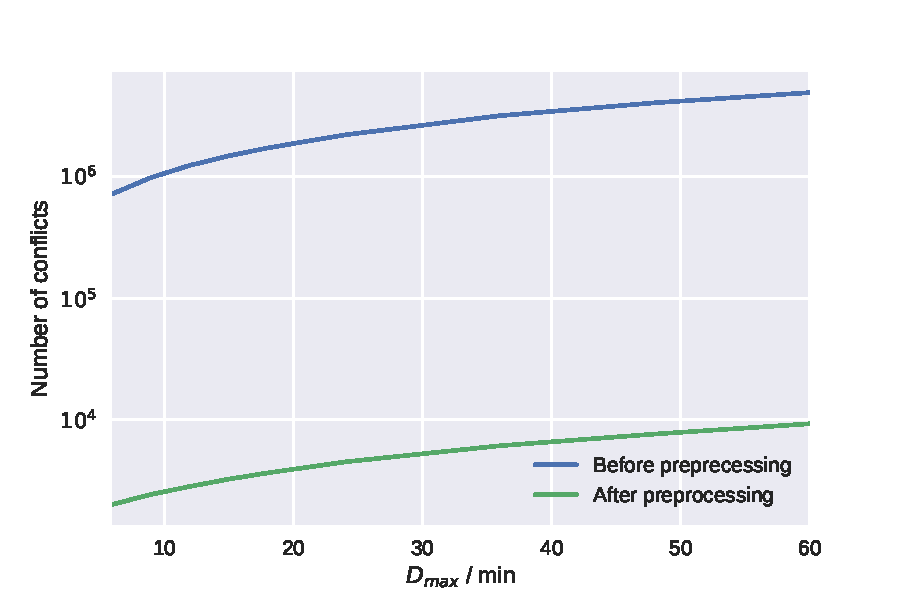
\includegraphics[width=0.45\textwidth]{./pics/preprocessing_reduction_number_of_conflicts.pdf}
    \end{center}
    \caption{Preprocessing: Reduction in the number of potential conflicts for various upper delay bounds $D_\text{max}$.}
\label{fig:preprocessing_reduction_number_of_conflicts}
\end{figure}

A conflict can be avoided locally by introducing earlier delays differentially, thereby increasing the temporal separation; by some active maneuver of one or both of the flights; or by some combination thereof.
We focus on the former case.
Let 
\begin{equation}
D_{i, k} = d_i + \sum_{\left.k' \in K_i \middle| k' < k\right.} d_{i,k'}
\end{equation}
be the accumulated delay of flight $i$ by the time it reaches conflict $k$.
We assume that the set of conflicts $K_i$ associated with flight $i$ is indexed in temporal order, i.e.\ if $k' < k$ and $k, k' \in K_i$, then flight $i$ reaches conflict $k'$ before conflict $k$.
The pairs of conflicting trajectory points associated with conflict $k$ are given by 
\begin{equation}
T_k = 
\left\{
(s, t) \middle| \{(i, s), (j, t)\} \in C_k, i < j
\right\}.
\end{equation}
Thus the potential conflict is avoided only if 
\begin{equation}
D_{i, k} - D_{j, k}
\notin
D_k 
\end{equation}
where 
\begin{align}
D_k &= 
\bigcup_{(s, t) \in T_k}
\left(-\Delta_t + t - s, \Delta_t + t - s\right)
=
[\Delta^{\min}_k, \Delta^{\max}_k], \\
\Delta^{\min}_k &= 1 - \Delta_t + \min_{(s, t) \in T_k} \{t - s\},\\
\Delta^{\max}_k &= \Delta_t - 1 + \max_{(s, t) \in T_k} \{t - s\}.
\end{align}

%In the absence of active maneuvers to avoid conflicts, the deconflicting problem can be summarized as minimizing the total delay $D$ subject to

In the remainder of this paper, we focus on the restricted problem in which only departure delays are allowed.
In this simplified case, the configuration space is simply 
$\mathbf d = {\left(d_i\right)}_{i=1}^n$, the cost function simply $D = \sum_{i = 1}^n d_i$, and the constraints simply $d_i - d_j \not in D_k$ for all $k$.
